\documentclass[11pt, oneside, titlepage]{article}
\usepackage[letterpaper, margin=2cm]{geometry}
\usepackage{MATH517}
\usepackage{Calculus}

\title{MATH 517 Finite Differences Homework 3}
\author{Caleb Logemann}

\begin{document}
\maketitle
%\noindent \textbf{\Large{Caleb Logemann \\
%MATH 517 Finite Difference Methods \\
%Homework 2
%}}

%\lstinputlisting[language=Matlab]{H01_23.m}
\begin{enumerate}
    \item % #1 Done
        Consider Poisson's equation in 2D:
        \begin{align*}
            -u_{xx} - u_{yy} = f(x,y)\text{ in } \Omega = \br{0, 1} \times \br{0, 1} \\
            u = g(x,y)\text{ on } \partial\Omega
        \end{align*}
        Discretize this equation using the 9-point Laplacian on a uniform mesh
        $\Delta x = \Delta y = h$.
        Use the standard row-wise ordering.

        First we need to specify the discretization of the space $\Omega$.
        Let $x_i = ih$ for $i = 0, 1, \ldots, N+1$ and let $y_j = jh$ for
        $j = 0, 1, \ldots, N+1$, where $h = \frac{1}{N+1}$.
        Then the solution to this PDE can be described by approximating u on
        this mesh, that is $U_{i,j} \approx u(x_i, y_j)$ is an approximation
        to the exact solution.

        Now we can apply finite differences to this PDE.
        The 9-point Laplacian on a uniform mesh is given by 
        \[
            \Delta_9 u = \frac{1}{6h^2}\p{U_{i-1,j-1} + U_{i-1,j+1} +
            U_{i+1,j-1} + U_{i+1,j+1} + 4U_{i-1,j} + 4U_{i+1,j} + 4U_{i,j-1} + 4U_{i,j+1} - 20U_{i,j}}.
        \]
        It can be shown that 
        \[
            \Delta_9 u = \Delta u + \frac{h^2}{12}\Delta f + O(h^4).
        \]

        Using this finite difference in the PDE results in the following set
        of equations that include the Laplacian of the forcing function.
        \begin{align*}
            \frac{1}{h^2}\p{20U_{i,j} - 4U_{i-1,j} - 4U_{i+1,j} - 4U_{i,j-1} -
            4U_{i,j+1} - U_{i-1,j-1} - U_{i-1,j+1} - U_{i+1,j-1} - U_{i+1,j+1}} \\
            = f_{ij} + \frac{h^2}{2} \Delta f_{ij}
        \end{align*}
        where $f_{ij} = f(x_i, y_j)$ and $\Delta f_{ij} = \Delta f(x_i, y_j)$.

        Now in order to turn this into a linear system, a new numbering scheme
        needs to be imposed.
        I will use the natural row-wise ordering where each point is numbered
        along the rows starting at $U_{1,1} = U_1$.
        In general $U_k = U_{i,j}$ when $k = i + (j-1)N$.

        Using this numbering scheme, the finite difference method turn into the
        following linear system.
        \begin{align*}
            A\v{U} &= \v{f}
            \intertext{$A \in \RR^{N^2 \times N^2}$ is the block matrix}
            A &=
            \begin{bmatrix}
                T  &  S     &        &        &    \\
                 S &  T     &  S     &        &    \\
                   & \ddots & \ddots & \ddots &    \\
                   &        &      S &      T &  S \\
                   &        &        &      S &  T
            \end{bmatrix} \\
            T &= 
            \begin{bmatrix}
                20 & -4     &        &        &    \\
                -4 & 20     & -4     &        &    \\
                   & \ddots & \ddots & \ddots &    \\
                   &        &     -4 &     20 & -4 \\
                   &        &        &     -4 & 20
            \end{bmatrix} \\
            S &= 
            \begin{bmatrix}
                -4 & -1     &        &        &    \\
                -1 & -4     & -1     &        &    \\
                   & \ddots & \ddots & \ddots &    \\
                   &        &     -1 &     -4 & -1 \\
                   &        &        &     -1 & -4
            \end{bmatrix} \\
            \v{f} &=
            \begin{bmatrix}
                6h^2 f(x_1, y_1) + h^4/2 \Delta f(x_1, y_1) + g(x_1,y_0) + g(x_0, y_1)\\
                6h^2 f(x_2, y_1) + h^4/2 \Delta f(x_2, y_1) + g(x_2, y_0) \\
                \vdots   \\
                6h^2 f(x_{N-1}, y_N) + h^4/2 \Delta f(x_{N-1}, y_N) + g(x_{N-1}, y_{N+1})  \\
                6h^2 f(x_N, y_N) + h^4/2 \Delta f(x_N, y_N) + g(x_{N+1}, y_N) + g(x_N, y_{N+1})
            \end{bmatrix}
        \end{align*}
        For the vector $\v{f}$ the boundary conditions are present for any
        index $k$ that appears on the boundary of the mesh, otherwise
        the entry of $\v{f}$ is simply $6h^2 f(x_i, y_j) + h^4/2 \Delta f(x_i, y_j)$.

    \item % #2 Done
        Write a MATLAB code that constructs the sparse coefficient matrix $A$
        and the appropriate right-hand side vector $\v{F}$.
        NOTE: you will need to modify the right-hand side vector to include
        the appropriate Laplacian of the right-hand side function.

        The following code is a function that solve the 2D Poisson problem
        using the 9 Point Laplacian.
        \lstinputlisting[language=Matlab]{Poisson2D_9PointLaplacian.m}

    \item % #3 Done
        Using your code do a numerical convergence study for the following
        right-hand side forcing and exact solution:
        \begin{align*}
            f(x,y) = -1.25e^{x + .5y}\quad\text{and}\quad u(x,y) = e^{x + .5y}
        \end{align*}
        Just use the built-in backslash operator in MATLAB to solve the linear
        system.

        The following script uses the previous function to test the convergence.
        \lstinputlisting[language=Matlab]{H03_2.m}
        The scripts output is as follows.
        \begin{verbatim}
            >> H03_2

            ans = 

                hRatios    errorRatios     order 
                _______    ___________    _______

                2          15.904          3.9914
                2          15.964          3.9968
                2          15.929          3.9936
                2          12.734          3.6706
                2          1.3226         0.40343
        \end{verbatim}

    \item % #4 Done
        Discretize the above PDE using the 5-point Laplacian.
        Write a MATLAB code that generates the sparse coefficient matrix $A$
        for this discretization.

        This PDE can be discretized very similary to the square geometry with
        the 5-point Laplacian.
        In fact I will begin with the same discretization as in that problem
        which uses the natural row-wise ordering.
        To recall this discretization resulted in the following
        linear algebra problem.
        \begin{align*}
            A\v{U} &= \v{f}
            \intertext{$A \in \RR^{N^2 \times N^2}$ is the block matrix}
            A &=
            \begin{bmatrix}
                T  & -I     &        &        &    \\
                -I &  T     & -I     &        &    \\
                   & \ddots & \ddots & \ddots &    \\
                   &        &     -I &      T & -I \\
                   &        &        &     -I &  T
            \end{bmatrix} \\
            T &= 
            \begin{bmatrix}
                4  & -1     &        &        &    \\
                -1 &  4     & -1     &        &    \\
                   & \ddots & \ddots & \ddots &    \\
                   &        &     -1 &      4 & -1 \\
                   &        &        &     -1 &  4
            \end{bmatrix}
            \intertext{and $I$ is the $N \times N$ identity matrix}
            \v{f} &=
            \begin{bmatrix}
                h^2 f(x_1, y_1) + g(x_1,y_0) + g(x_0, y_1)\\
                h^2 f(x_2, y_1) + g(x_2, y_0) \\
                \vdots   \\
                h^2 f(x_{N-1}, y_N) + g(x_{N-1}, y_{N+1})  \\
                h^2 f(x_N, y_N) + g(x_{N+1}, y_N) + g(x_N, y_{N+1})
            \end{bmatrix}
        \end{align*}

        Now when considering the differences between the square geometry and
        the L-shaped geometry, it is clear that the only difference is that
        some discretization points now lie outside of the geometry or on the
        boundary.
        In order to take this into account, if $U_i$ lies outside the L-shaped
        geometry, we can change the old equation governing this point to $U_i = 0$.
        This changes the matrix $A$ so that the ith row is all zeros except
        for a 1 on the diagonal.
        In other words $A_{ii} = 1$ and $A_{ij} = 0$ for $j \neq i$.
        The other change that needs to take place is that now
        $U_i$ cannot have a weight for any other nodes equation.
        This changes $A$ so that the ith column is all zeroes except for the
        diagonal.
        Thus $A_{ii} = 1$ as before and $A_{ji} = 0$ for $j \neq i$.
        In essence the rows and columns corresponding to the points outside
        the L-shaped geometry are zeroed out.
        They are then replaced with equations settings these points to zero.

        The final difference between this problem and the previous square
        geometry, is that the boundary conditions are set to zero.
        This means that $g(x,y) = 0$ for all points on the boundary.
        This difference is reflected in the right-hand side vector.

        Lastly we need to identify the points outside the L-shaped geometry.
        First note that $N$ must be odd so that discretization points lie on
        the boundaries at $x = .5$ and $y = .5$.
        Since $N$ is odd, there exists some positive integer $m$ such that
        $N = 2m + 1$.
        This integer $m$ can be thought of as the number of discretization
        points between $y = 0$ and $y = .5$ or $x = .5$ and $x = 1$.
        The points on the boundary at $y = .5$ from $x = 0$ to $x = .5$ start
        with $mN + 1$ and end with $mN + 1 + m$.
        For rows $m + 1$ to $N$ the first $m + 1$ points are not part of the geometry.
        Therefore indices of the form $mi + j$ for $i = m+1, m+2, \ldots, N$ and
        $j=1, 2, \ldots m + 1$ are not included in the geometry.

        All of these chages results in the following linear algebra problem.
        \begin{align*}
            A\v{U} &= \v{f}
            \intertext{$A \in \RR^{N^2 \times N^2}$ is the block matrix}
            A &=
            \begin{bmatrix}
                T  & -I     &        &        &    \\
                -I &  T     & -I     &        &    \\
                   & \ddots & \ddots & \ddots &    \\
                   &        &   -I_n &    T_n & -I_n \\
                   &        &        &   -I_n &  T_n
            \end{bmatrix} \\
            T &= 
            \begin{bmatrix}
                4  & -1     &        &        &    \\
                -1 &  4     & -1     &        &    \\
                   & \ddots & \ddots & \ddots &    \\
                   &        &     -1 &      4 & -1 \\
                   &        &        &     -1 &  4
            \end{bmatrix} \\
            T_n &= 
            \begin{bmatrix}
                1  &  0     &        &        &    \\
                 0 &  1     & 0      &        &    \\
                   & \ddots & \ddots & \ddots &    \\
                   &        &     -1 &      4 & -1 \\
                   &        &        &     -1 &  4
            \end{bmatrix} \\
            I_n &= 
            \begin{bmatrix}
                0  &        &        &        &    \\
                   &  0     &        &        &    \\
                   &        & \ddots &        &    \\
                   &        &        &      1 &    \\
                   &        &        &        &  1
            \end{bmatrix}
            \intertext{and $I$ is the $N \times N$ identity matrix}
            \v{f} &=
            \begin{bmatrix}
                h^2 f(x_1, y_1) \\
                h^2 f(x_2, y_1) \\
                \vdots \\
                h^2 f(x_{N-1}, y_N) \\
                h^2 f(x_N, y_N)
            \end{bmatrix}
        \end{align*}
        In this case $T_n$ and $I_n$ make up the lower half of the diagonal, for
        the $m + 1$ block and onward.
        In $T_n$ the upper half is only 1s on the diagonal, the lower half is
        identical to $T$.
        $I_n$ is zero on the digaonal for $i \le m + 1$, and the identity otherwise.
        The discretization is implemented in the following function.
        \lstinputlisting[language=Matlab]{Poisson2D_5PointLaplacian_IrregularGeometry.m}

    \item % #5 Done
        For $N = 19$ and $N = 39$ produce a spy plot of the matrix.
        \begin{center}
            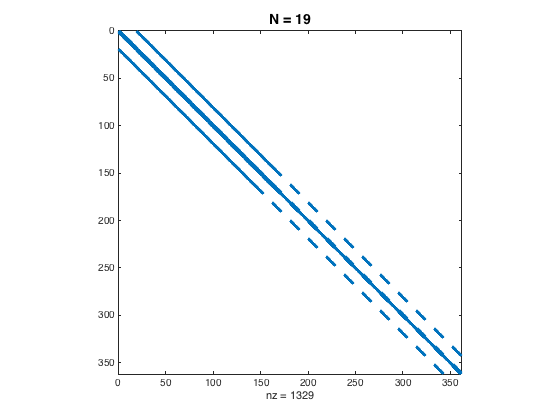
\includegraphics[scale=.5]{Figures/03_5_1.png}
            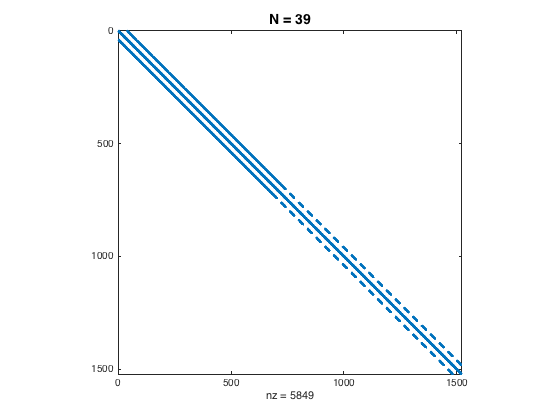
\includegraphics[scale=.5]{Figures/03_5_2.png}
        \end{center}

    \item % #6 Done
        Solve the PDE using your code with the right hand side
        \[
            f(x, y) = 1.
        \]

        The following code evalates the function from problem 4 for the
        given right hand side.
        The images produced are shown below.
        \lstinputlisting[language=Matlab, lastline=12]{H03_4.m}
        \begin{center}
            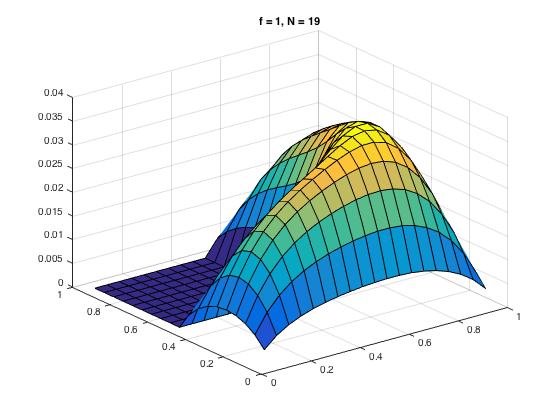
\includegraphics[scale=.5]{Figures/03_6_1.png}
            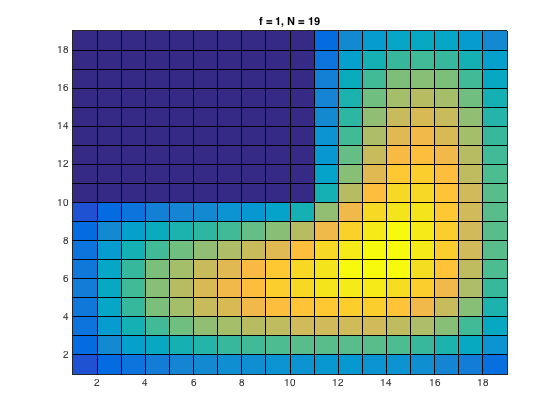
\includegraphics[scale=.5]{Figures/03_6_2.png}
            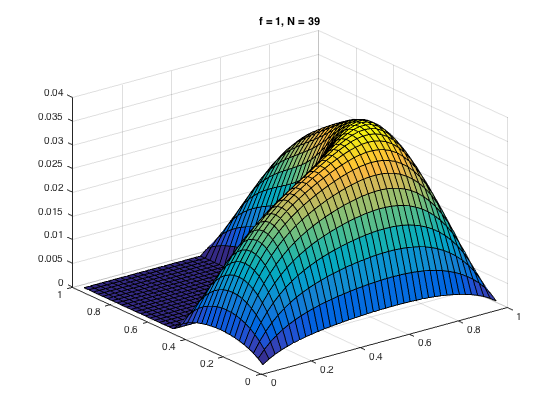
\includegraphics[scale=.5]{Figures/03_6_3.png}
            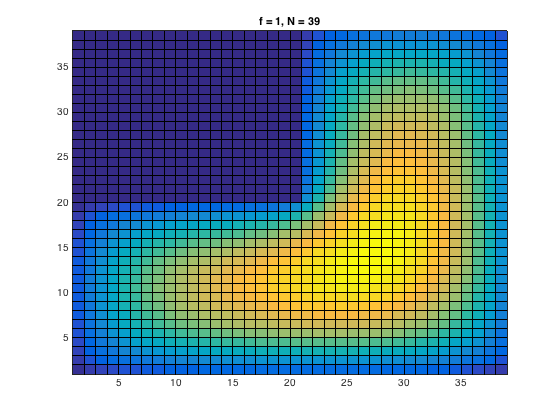
\includegraphics[scale=.5]{Figures/03_6_4.png}
        \end{center}

    \item % #7 Done
        Solve the PDE using your code with the right hand side
        \[
            f(x, y) = 2 exp\br{-(10x - 5)^2 - (10y - 5)^2}.
        \]

        The following code evalates the function from problem 4 for the
        given right hand side.
        The images produced are shown below.
        \lstinputlisting[language=Matlab, firstline=14, lastline=25]{H03_4.m}
        \begin{center}
            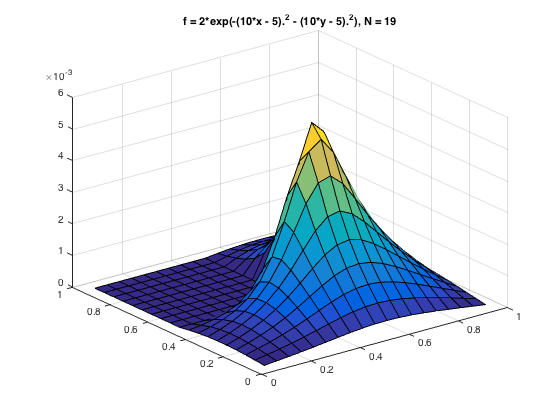
\includegraphics[scale=.5]{Figures/03_7_1.png}
            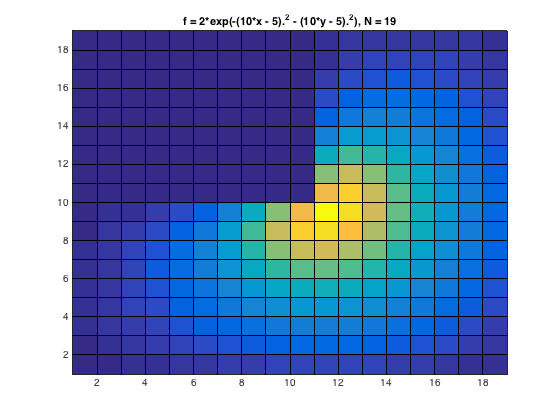
\includegraphics[scale=.5]{Figures/03_7_2.png}
            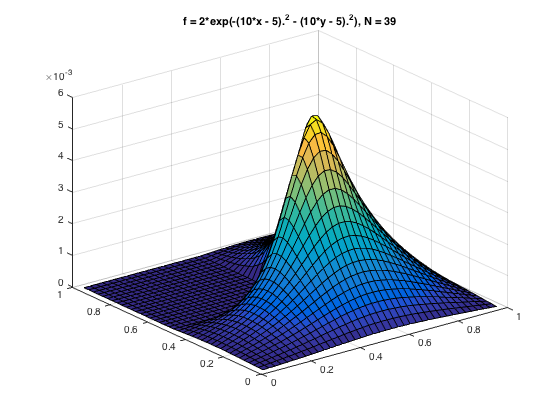
\includegraphics[scale=.5]{Figures/03_7_3.png}
            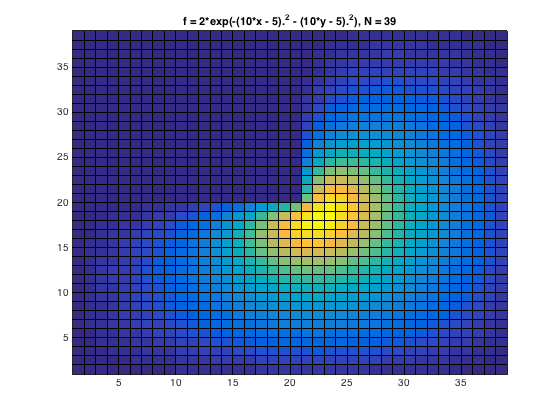
\includegraphics[scale=.5]{Figures/03_7_4.png}
        \end{center}

    \item % #8 Done
        Compute the Cholesky factorization of A is MATLAB: R = chol(A);
        where $R$ is an upper triangular matrix such that $A = R^T R$.
        For $N = 19$ and $N = 39$ produce a spy plot of $R$.
        Create a table showing the non-zeros in R for
        $N = 9, 19, 39, 79, 159, 319$.

        The following code is for problems 8 and 9.
        \lstinputlisting[language=Matlab, firstline=27]{H03_4.m}

        The following is the spy plots and table for problem 8.
        \begin{center}
            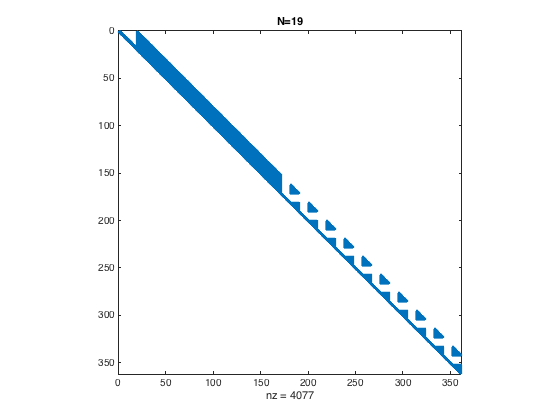
\includegraphics[scale=.5]{Figures/03_8_1.png}
            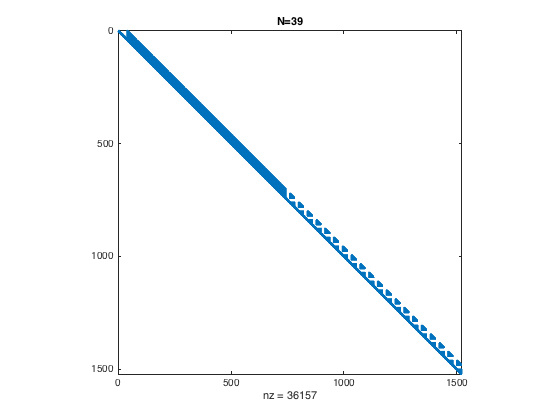
\includegraphics[scale=.5]{Figures/03_8_2.png}
        \end{center}

        \begin{verbatim}
            ans = 

                Var1     countsA  
                ____    __________

                9            412
                19           4077
                39          36157
                79     3.0432e+05
                159     2.4966e+06
                319     2.0225e+07
        \end{verbatim}

    \item % #9 Done
        Permute the matrix $A$ using the reverse Cuthill-Mckee algorithm in
        MATLAB: P = symrcm(A); B = A(P, P);
        Compute the Cholesky factorization of $B$ in MATLAB: R = chol(B);
        For $N = 19$ and $N = 39$ produce a spy plot of $R$.
        Create a table showing the non-zeros in R for
        $N = 9, 19, 39, 79, 159, 319$.

        The following is the spy plots and table for problem 9 generated by
        the code shown under problem 8.
        \begin{center}
            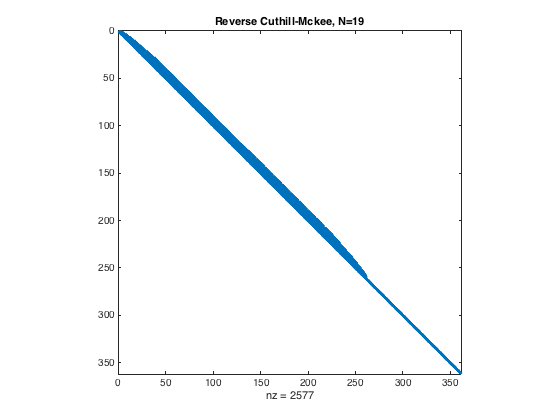
\includegraphics[scale=.5]{Figures/03_9_1.png}
            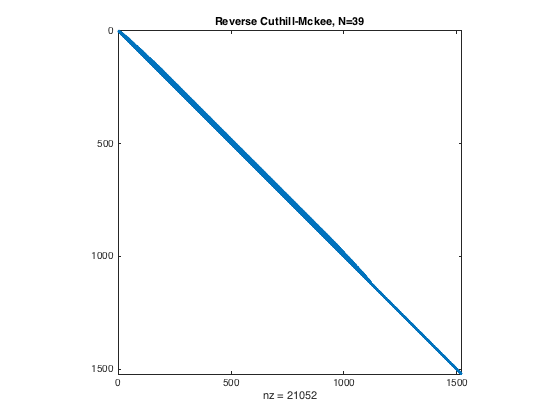
\includegraphics[scale=.5]{Figures/03_9_2.png}
        \end{center}
        \begin{verbatim}
            ans = 

                Var1     countsB  
                ____    __________

                9            302
                19           2577
                39          21052
                79      1.697e+05
                159     1.3618e+06
                319     1.0909e+07
        \end{verbatim}
\end{enumerate}
\end{document}
